% This file was created by matplotlib2tikz v0.7.4.
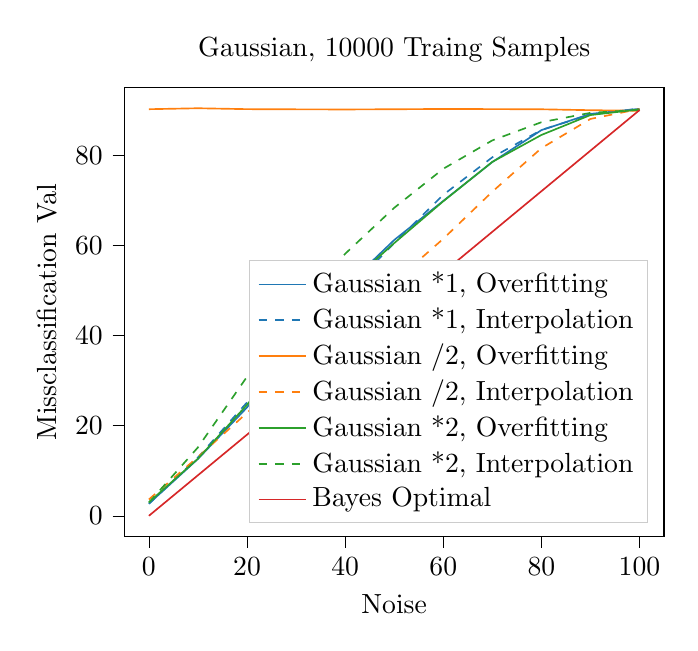
\begin{tikzpicture}

\definecolor{color0}{rgb}{0.12156862745098,0.466666666666667,0.705882352941177}
\definecolor{color1}{rgb}{1,0.498039215686275,0.0549019607843137}
\definecolor{color2}{rgb}{0.172549019607843,0.627450980392157,0.172549019607843}
\definecolor{color3}{rgb}{0.83921568627451,0.152941176470588,0.156862745098039}

\begin{axis}[
legend cell align={left},
legend style={at={(0.97,0.03)}, anchor=south east, draw=white!80.0!black},
tick align=outside,
tick pos=left,
title={Gaussian, 10000 Traing Samples},
x grid style={white!69.01960784313725!black},
xlabel={Noise},
xmin=-5, xmax=105,
xtick style={color=black},
y grid style={white!69.01960784313725!black},
ylabel={Missclassification Val},
ymin=-4.5205, ymax=94.9305,
ytick style={color=black}
]
\addplot [semithick, color0]
table {%
0 2.7
10 12.62
20 24.04
30 39.04
40 50.73
50 61.18
60 69.85
70 78.48
80 85.55
90 89.16
100 90.28
};
\addlegendentry{Gaussian *1, Overfitting}
\addplot [semithick, color0, dashed]
table {%
0 2.66
10 12.94
20 25.16
30 37.02
40 49.26
50 60.5
60 71.2
70 79.53
80 85.6
90 89.02
100 90.35
};
\addlegendentry{Gaussian *1, Interpolation}
\addplot [semithick, color1]
table {%
0 90.2
10 90.41
20 90.21
30 90.17
40 90.14
50 90.19
60 90.25
70 90.22
80 90.18
90 89.98
100 89.85
};
\addlegendentry{Gaussian /2, Overfitting}
\addplot [semithick, color1, dashed]
table {%
0 3.63
10 13.06
20 22.84
30 32.4
40 42.14
50 51.89
60 61.45
70 71.9
80 81.55
90 88.04
100 90.24
};
\addlegendentry{Gaussian /2, Interpolation}
\addplot [semithick, color2]
table {%
0 3
10 12.68
20 24.63
30 38.26
40 50.76
50 60.49
60 69.77
70 78.51
80 84.48
90 88.9
100 90.15
};
\addlegendentry{Gaussian *2, Overfitting}
\addplot [semithick, color2, dashed]
table {%
0 2.92
10 15.18
20 30.85
30 45.29
40 58.12
50 68.32
60 76.98
70 83.28
80 87.31
90 89.39
100 90.06
};
\addlegendentry{Gaussian *2, Interpolation}
\addplot [semithick, color3]
table {%
0 0
10 9
20 18
30 27
40 36
50 45
60 54
70 63
80 72
90 81
100 90
};
\addlegendentry{Bayes Optimal}
\end{axis}

\end{tikzpicture}